\documentclass[doublespace,Afour,sageh,times]{sagej}
\usepackage{amsmath,amssymb,amsthm,graphicx,booktabs,array,url}
\usepackage{xr-hyper}
\usepackage[colorlinks,bookmarksopen,bookmarksnumbered,citecolor=blue,urlcolor=blue]{hyperref}
\setcounter{secnumdepth}{3}
\setcounter{dbltopnumber}{2}
\renewcommand{\dbltopfraction}{0.85}
\def\journalname{The International Journal of Robotics Research}
\runninghead{Complex Hamiltonian learning and KAM stability}
\newtheorem{theorem}{Theorem}
\newtheorem{proposition}[theorem]{Proposition}
\newtheorem{lemma}[theorem]{Lemma}
\newtheorem{corollary}[theorem]{Corollary}
\theoremstyle{definition}
\newtheorem{assumption}{Assumption}
\newtheorem{remark}{Remark}
\newcommand{\R}{\mathbb R}
\newcommand{\C}{\mathbb C}
\newcommand{\T}{\mathbb T}
\newcommand{\dd}{\,\mathrm d}
\newcommand{\norm}[1]{\left\lVert#1\right\rVert}
\newcommand{\abs}[1]{\left|#1\right|}
\newcommand{\diag}{\operatorname{diag}}
\newcommand{\Rea}{\operatorname{Re}}
\newcommand{\Ima}{\operatorname{Im}}
\newcommand{\eps}{\varepsilon}
\providecommand{\doi}[1]{\href{https://doi.org/#1}{doi: #1}.}

\externaldocument[S-]{supplement}
\begin{document}
\title{Complex Hamiltonian learning and KAM-preserving magnetic control of a catheter model}
\author{Anonymous authors}
\begin{abstract}
A learned model of a magnetic catheter should connect accurate prediction to bounded motion and realizable actuation. We develop this connection for a clamped--free beam in four steps. First, we derive its complex Hamiltonian representation and the complete fourth-order central symplectic update. Second, matched learning and integration comparisons quantify approximation and numerical errors. Third, nonzero-loss, state-only two-mode COMSOL identification yields coefficient and analytic-error bounds that support an a posteriori KAM proof for the fitted Hamiltonian at approximately $1.9$ mm amplitude. Fourth, magnetic force-and-torque feedback realizes that conservative motion in the damped $64$-mode plant. For zero higher-mode startup, the whole-centreline bound is below $1.971$ mm. An input-work constraint additionally guarantees clearance during driven motion, including a quantified nonzero-error envelope over $4$ s. Frequency continuation resolves a resonance-induced clearance boundary, and an S-shaped endpoint task achieves $6.419\,\mu$m RMS tracking error. Classical symplectic and KAM results underpin the analysis; the contributions are the model-specific error bounds, magnetic realization and full-model motion guarantees under stated sensing and actuation assumptions.
\end{abstract}
\keywords{magnetic catheter robots, complex Hamiltonian learning, symplectic integration, KAM theory, magnetic control}
\maketitle
\raggedbottom
\section{Background and research question}
\label{sec:background}
Magnetic actuation can steer a flexible catheter without placing motors along its body. A field applies torque to a magnetic segment, and a field gradient can supply force; elastic deformation and dissipation then determine the motion of the entire device \citep{abbott,kim}. For operation inside a confined passage, a useful dynamical model must therefore do more than predict the tip. It must connect available magnetic inputs to bounded centreline motion. This paper develops that connection for a clamped--free catheter model, using a learned Hamiltonian as the common object for numerical integration, nonlinear stability analysis and feedback design.

The application motivation is remote manipulation in reduced gravity. Spaceflight creates medical and operational conditions that warrant dedicated investigation; NASA's assessment of spaceflight-associated neuro-ocular syndrome is one example of a gravity-dependent health risk \citep{nasa}. For a remotely manipulated device in this setting, we isolate the following mechanical question: how to sustain a prescribed class of bounded motions and respect a clearance limit when a flexible magnetic device has distributed inertia, elasticity and damping. The model is planar, has small slopes and neglects gravity and contact. These assumptions make the energy balance explicit and permit independent finite-element calculations, while identifying the physical effects that a later device study must supply.

Two operating objectives organize the analysis. The first is recurrent motion with a proved amplitude bound, represented by an invariant torus of a conservative model. The second is tracking a requested endpoint path while keeping the intervening body inside a corridor. The first objective asks whether motion persists for arbitrarily long times; the second asks how much external work can safely be supplied during a manoeuvre. A common mechanical energy links them, but they call for different conclusions. We use KAM theory for the recurrent motion and an input-work inequality for clearance, then derive magnetic commands that make those conclusions relevant to the same damped beam.

The main difficulty is preserving this connection through learning and actuation. Low prediction error alone leaves the Hamiltonian's nonlinear derivatives undetermined. Even with accurate derivatives, a numerical solver can introduce an error comparable to the difference between two learned models. Finally, damping removes the recurrent motion of a conservative system unless a controller supplies the appropriate work. We address these issues in sequence: construct a power-consistent learned energy, resolve its approximation and integration errors, establish an invariant motion of the fitted function, and realize that motion with the available magnetic force and torque.

Recent magnetic-robot control studies address shape regulation and lumen navigation directly. \citet{francescon2025shape} combine a pseudo-rigid-link model with vision feedback and homogeneous fields to control a robot with a prescribed lengthwise magnetization profile, demonstrating navigation in a soft pancreatic-duct phantom under varied insertion poses. \citet{tong2025navigation} use a geometrically nonlinear magnetic-rod simulation with reduced contact handling to compute fields that reduce distal-tip constraint forces, with planar phantom experiments and three-dimensional numerical demonstrations. These studies establish practical routes from a mechanical model to magnetic commands. The question pursued here is how a learned energy, with a quantified identification error, can support both persistent motion and bounds on the entire centreline. For the stated planar beam, we connect analytic error and twist bounds to a finite-amplitude invariant torus, realize its low-mode dynamics in the damped full finite-element plant, and bound driven motion through supplied work. Table~\ref{tab:core-roadmap} summarizes the objects passed between these steps.

\begin{table*}[t]
\centering
\caption{Four steps of the study. Each step supplies the object needed by the next; the detailed proofs and additional experiments are in the Supplement.}
\label{tab:core-roadmap}
\begin{tabular}{p{0.16\textwidth}p{0.29\textwidth}p{0.44\textwidth}}
\toprule
Step & Question & Result passed to the next step\\
\midrule
1. Derive, Section~\ref{sec:derivation} & Which energy and discrete update describe the beam? & A power-consistent complex representation and a complete central symplectic update.\\
2. Evaluate, Section~\ref{sec:analysis} & What errors remain after fitting and integration? & Paired comparisons and quantitative approximation bounds for a specified learned function.\\
3. Establish persistence, Section~\ref{sec:kam} & Does that function preserve a nonlinear recurrent motion? & Nondegenerate twist, a finite-amplitude invariant torus and a local family of tori.\\
4. Realize, Section~\ref{sec:application} & How does the motion guide magnetic actuation? & Force/torque feedback, full-model amplitude bounds and clearance-constrained tracking.\\
\bottomrule
\end{tabular}
\end{table*}

\subsection{Learning a mechanical model that can be analyzed}
The starting point is a mechanical energy with explicit boundary work. Variational beam and rod formulations relate distributed strain energy, inertia and applied loads before discretization \citep{simo,antman}. In the present specialization, the tip magnet contributes a cosine potential under a static bias field. Its curvature enters the linear modal frequencies, while its higher-order terms govern the amplitude dependence of those frequencies. We retain the complete cosine because the nonlinear part later supplies the twist required for KAM nondegeneracy. Modal coordinates are normalized once, and the same dimensional map is used to interpret learned coefficients, simulated trajectories and magnetic commands. Supplement~\ref{S-sec:mechanics} supplies the distributed derivation; Section~\ref{sec:derivation} develops the model used in the analysis.

Hamiltonian neural networks provide a natural learning mechanism: fit a scalar energy and obtain its canonical vector field by differentiation \citep{greydanus}. This makes the energy derivatives available to both numerical integration and stability analysis. A magnetic catheter also loses and receives energy, so we follow the separation of conservative dynamics, dissipation and inputs used by dissipative SymODEN and port-Hamiltonian networks \citep{zhong,desai}. The learned conservative part specifies reversible dynamics; a nonnegative dissipation model and explicit magnetic ports complete the physical decoder. This separation is necessary for a controller to distinguish the energy stored by the device from the work it must supply.

Complex coordinates package modal position and momentum into one state. This representation supports shared complex features \citep{trabelsi}. Their physical interpretation remains tied to the underlying real energy. We derive that representation explicitly, including the conjugate dependence and the analytic extension used in the KAM argument. Complex-network approximation theory offers useful existence and comparison results, but those results depend on the activation, target class and norm \citep{zhang}. Here the relevant question is whether the fitted model controls the required derivatives on a declared domain. Smooth approximation theory \citep{hornik} provides an existence route; the quantitative analysis then uses the actual finite feature class and its fitted coefficients.

That feature class combines the complete magnetic potential with an analytic polynomial residual. Its coefficients can be fitted from energy derivatives or state increments, and all derivatives needed for the subsequent analysis are explicit. A residual may depend on momentum as well as position. We retain that dependence because it changes both the Hamiltonian vector field and the relation between physical velocity and canonical momentum. The magnetic feedback is consequently derived from the full learned gradient and Hessian. This gives learning a concrete role: it supplies a differentiable energy whose approximation error can be bounded and whose dynamics can be translated back into physical commands.

The distinction between identification and model reduction is particularly important for this device. A low-mode projection of a full beam trajectory need not satisfy a closed low-mode equation: the discarded modes also contribute to tip rotation and hence magnetic torque. A fitted residual can absorb part of that discrepancy on the observed trajectories. Its predictive value should therefore be assessed against independent full-beam solutions, while a theorem about that residual must use the function actually obtained by fitting. We organize the computations around both questions. Controlled reduced-model data isolate coefficient recovery and permit a quantitative learning-to-KAM argument. Independent full finite-element observations assess the discrepancy introduced by reduction and the response to driven motion.

The comparison design separates the effects of representation and mechanical knowledge. Real and complex implementations are fitted with and without the known quadratic energy, using paired training seeds and the same held-out trajectories. Five paired contrasts measure the effect of the prior in each representation, the representation effect with and without that prior, and their interaction. A separate integration comparison resolves numerical error before small learning differences are interpreted. The resulting real and complex predictions are equivalent at the resolved precision for this feature class.

\subsection{From numerical trajectories to persistent physical motion}
A learned Hamiltonian is continuous in time, whereas prediction and control require discrete updates. Central generating functions provide classical symplectic difference schemes for this step \citep{feng}. We derive the fourth-order central formula through its midpoint expansion and specialize it to the fitted magnetic energy. The correction, its symplecticity and its order belong to the established geometric-integration framework \citep{hairer}; the model-specific work is the complete realization for the learned, generally nonseparable Hamiltonian and its numerical evaluation. This treatment exposes the derivatives actually required by the update and allows the solver tolerance, phase error and state error to be assessed together.

The resulting numerical trajectories motivate the stability question, but KAM persistence is determined by properties of the Hamiltonian itself. Classical KAM theory connects sufficiently small perturbations of nondegenerate integrable systems to families of invariant tori \citep{poschel,bounemoura}. For the magnetic beam, the nonlinear frequency variation can be computed from the retained cosine. Learning must preserve that variation and control the full remainder. The analysis therefore follows coefficients and analytic norms through to the theorem assumptions.

Chen et al. connect nonzero Hamiltonian-network training loss to KAM theory under statistical and regularity hypotheses \citep{chen2022}. We develop a computable counterpart for the present analytic feature class. In the experiment used for the finite-amplitude proof, state-only COMSOL observations determine an integral regression. Bounds on its residual, integration defect and design matrix yield a coefficient-error bound; differentiating the same features converts it into analytic-error and twist bounds. Thus the learning error remains part of the argument even though the training loss is nonzero. The broader statistical route is retained in Supplement~\ref{S-sec:transfer}, while the main proof uses the deterministic bounds appropriate to these trajectory observations.

With those bounds in place, an a posteriori KAM theorem tests a computed torus of the fitted Hamiltonian through its invariance defect and geometric conditions \citep{haro2019aposteriori}. We apply it to the exported learned function, including its complete cosine and momentum-dependent residual. The result is a torus at approximately $1.9$ mm amplitude. Nondegeneracy of its final torsion also supplies a local family of positive measure through an established torus-stability result \citep{bounemoura2016torus}. Explicit measure estimates require a specified domain and constants \citep{biasco2018measure,chierchia2021measure}; we retain that calculation in the Supplement. Weighted Birkhoff averages additionally explore a wider domain over finite times \citep{das2017quasiperiodicity,duignan2023flows}, providing a complementary numerical view of the recurrent motions.

For these motions to guide actuation, the conservative subsystem must be connected to the damped full beam. We use a transverse magnetic force and torque to reproduce the learned low-mode accelerations. The remaining modes then form stable forced oscillators, whose quasiperiodic responses can be constructed and bounded. This yields an invariant torus of the complete $64$-mode model and a bound that also includes startup from zero higher-mode states. Leaving the torus for an endpoint task invokes a second control mechanism: a magnetic-work governor limits physical energy and hence the whole-centreline deflection. The two mechanisms address recurrent operation and manoeuvring within the same mechanical setting.

\subsection{Contributions and study design}
The work contributes three model-specific results. First, it derives the complex magnetic Hamiltonian, implements the classical fourth-order central update for the learned nonseparable energy, and resolves representation, prior and integration effects through matched comparisons. Second, it converts nonzero state-only identification error into computable analytic and twist bounds, then verifies a finite-amplitude invariant torus of that fitted function. Third, it constructs magnetic feedback and a full-model torus lift, together with an energy-based clearance condition for driven motion. The general approximation and KAM theorems are established results, cited with their hypotheses and identifiers where applied; the coefficient bounds, mechanical constructions and application proofs are developed here.

The quantitative results make the connection operational within the stated model. Starting the low state on the certified torus and all higher states at zero gives a whole-centreline bound below $1.971$ mm, a transverse-field bound below $0.922$ mT and a gradient bound below $0.02573$ T/m. A separate S-shaped endpoint task achieves $6.419\,\mu$m RMS error with the learned controller.

Two COMSOL identification settings serve distinct purposes within this common mechanical model: full finite-element observations test prediction and tracking, whereas the two-mode integral observations supply the learning-to-KAM proof and the associated magnetic realization. Their fitted coefficients and error budgets are specified separately. Section~\ref{sec:conclusion} brings the results together.

\section{Derivation of the complex Hamiltonian and symplectic scheme}
\label{sec:derivation}
\subsection{From magnetic rod mechanics to canonical variables}
\label{sec:core-canonical-model}
We first derive an energy from magnetic beam mechanics, express that
energy in complex coordinates, and then discretize its conservative
flow. For a planar, small-slope cantilever, the transverse displacement
$w(s,t)$ satisfies
\begin{align}
 \rho A_c w_{tt}+c_d w_t+EIw_{ssss}&=0,\qquad 0<s<L,\nonumber\\
 w(0,t)=w_s(0,t)&=0,\qquad w_{sss}(L,t)=0,\nonumber\\
 EIw_{ss}(L,t)&=\mu[B_y\cos\vartheta-B_0\sin\vartheta],
 \label{eq:core-beam-balance}
\end{align}
where $\vartheta=w_s(L,t)$, $A_c=\pi r_c^2$, and $I=\pi r_c^4/4$.
The negative rotation derivative of the magnetic potential
$-\mu(B_0\cos\vartheta+B_y\sin\vartheta)$ gives the tip moment.
Thus the free-end rotation remains unconstrained, the constant bias
$B_0$ stores energy, and the transverse field $B_y(t)$ supplies work.

The $80$ mm beam has radius $0.6$ mm and uses $32$ consistent-mass
cubic-Hermite elements, leaving $64$ free coordinates after clamping;
supplementary Table~\ref{S-tab:unified-si} gives its material and field
parameters. Let $q$, $M$, $K$ and $e_\vartheta$ denote the nodal vector,
mass matrix, bending stiffness and tip-rotation selector. Two integrations
by parts in the Galerkin weak form place the natural moment on
$e_\vartheta$, giving the finite-element equations and stored energy
\begin{align}
 M\ddot q+\alpha M\dot q+Kq
 &=\mu e_\vartheta[B_y\cos\vartheta-B_0\sin\vartheta],\nonumber\\
 H_0(q,p)&=\tfrac12p^{\mathsf T}M^{-1}p+\tfrac12q^{\mathsf T}Kq\nonumber\\
 &\quad+E_0[1-\cos(e_\vartheta^{\mathsf T}q)],
 \label{eq:core-fe-energy}
\end{align}
where $p=M\dot q$, $E_0=\mu B_0=6.0\times10^{-7}\,\mathrm J$ and
$c_d=\alpha\rho A_c$, with $\alpha=0.55558524\,\mathrm{s^{-1}}$.
The cosine potential remains exact within the small-slope beam model.

The bias-field stiffness is $K_b=K+E_0e_\vartheta e_\vartheta^{\mathsf T}$.
Choose $\Phi_n^{\mathsf T}M\Phi_n=I$ and
$\Phi_n^{\mathsf T}K_b\Phi_n=\diag(\omega_j^2)$ for $n$ retained modes,
and write $q=\Phi_n a$, with reduced canonical momentum $\pi=\dot a$.
Set $\omega_0=\omega_1$, $\tau=\omega_0t$, and $\nu_j=\omega_j/\omega_0$.
Define the scalar position scales $S_j=\sqrt{E_0/(\omega_0\omega_j)}$.
The balanced scaling is
\begin{equation}
 a_j=\sqrt{\frac{E_0}{\omega_0\omega_j}}X_j,
 \qquad
 \pi_j=\sqrt{\frac{E_0\omega_j}{\omega_0}}Y_j.
 \label{eq:unified-scale}
\end{equation}
The scale product $E_0/\omega_0$, energy $H_0/E_0$ and time
$\tau=\omega_0t$ give canonical dimensionless equations.
Define $S=\Phi_n\diag(S_j)$,
$d=S^{\mathsf T}e_\vartheta$, and $\ell(s)^{\mathsf T}=N(s)S$, where
$N(s)$ is the Hermite displacement row. Then
$w(s)=\ell(s)^{\mathsf T}X$, $\vartheta=d^{\mathsf T}X$, and
\begin{align}
 h_*(X,Y)&=h_2(X,Y)+g(d^{\mathsf T}X),\nonumber\\
 h_2&=\tfrac12\sum_{j=1}^n\nu_j(X_j^2+Y_j^2),\nonumber\\
 g(s)&=1-\cos s-\tfrac12s^2.
 \label{eq:unified-h}
\end{align}
Subtracting $s^2/2$ avoids counting the bias stiffness twice.
For the two-mode learning model, $\omega_0\approx11.417287283\,\mathrm{rad\,s^{-1}}$,
$\nu\approx(1,6.152117504)$, $d\approx(0.225670773,0.321798806)^{\mathsf T}$,
and $\ell(L)\approx(0.013506054,0.005470926)^{\mathsf T}\,\mathrm m$.
Calculations use the full exported coefficients in this fixed chart,
shared by learning, integration and stability analysis.

\subsection{Complex energy and a power-consistent decoder}
\label{sec:core-complex-decoder}
The complex Hamiltonian follows by an invertible change of coordinates.
Let $x=(X,Y)\in\mathbb R^{2n}$,
$J=\left(\begin{smallmatrix}0&I\\-I&0\end{smallmatrix}\right)$, and
\begin{align}
 \zeta_j&=\frac{X_j+\mathrm iY_j}{\sqrt2},\qquad
 \chi_j=\frac{X_j-\mathrm iY_j}{\sqrt2},\nonumber\\
 X_j&=\frac{\zeta_j+\chi_j}{\sqrt2},\qquad
 Y_j=\frac{\zeta_j-\chi_j}{\mathrm i\sqrt2}.
 \label{eq:core-complex-chart}
\end{align}
On the real phase space $\chi=\bar\zeta$. Substitution into
\eqref{eq:unified-h} gives the explicit complex form
\begin{align}
 h_*^{\mathbb C}(\zeta,\chi)
 &=\sum_j\nu_j\zeta_j\chi_j
   +1-\cos\!\left(\frac{d^{\mathsf T}(\zeta+\chi)}{\sqrt2}\right)\nonumber\\
 &\quad-\tfrac14[d^{\mathsf T}(\zeta+\chi)]^2.
 \label{eq:core-complex-energy}
\end{align}
It restricts to the real energy when $\chi=\bar\zeta$ and is entire
in the independent complex variables $(\zeta,\chi)$. This extension,
including the learned polynomial residual below, supplies the analytic
Hamiltonian used in KAM theory. It need not be holomorphic in $\zeta$
alone. For a real analytic energy $h$, the chain rule yields
\begin{align}
 \{\zeta_j,\bar\zeta_k\}&=-\mathrm i\delta_{jk},\qquad
 \partial_{\bar\zeta_j}&=
       \frac{\partial_{X_j}+\mathrm i\partial_{Y_j}}{\sqrt2},\nonumber\\
 \zeta'&=-\mathrm i\partial_\chi h^{\mathbb C},\qquad
 \chi'=\mathrm i\partial_\zeta h^{\mathbb C}.
 \label{eq:core-complex-canonical}
\end{align}

Magnetic actuation and damping enter through the physical decoder.
A CHNN supplies real readouts $h_\eta$ and $\mathcal D_\eta(X,v)$,
with physical dissipation divided by $E_0\omega_0$, and
\begin{align}
 X'&=v=\partial_Yh_\eta,\nonumber\\
 Y'&=-\partial_Xh_\eta-\partial_v\mathcal D_\eta(X,v)
       +u\,d\cos(d^{\mathsf T}X).
 \label{eq:fragment-decoder}
\end{align}
Here $u=B_y/B_0$, and $\partial_v\mathcal D_\eta$ is evaluated before
substituting $v=\partial_Yh_\eta$. With $\mathsf N=\diag(\nu_j)$, we use
$\mathcal D_\eta=\widehat\gamma v^{\mathsf T}\mathsf N^{-1}v/2$,
$\widehat\gamma\ge0$; for the stated beam, $\gamma=\alpha/\omega_0$.
Taking the derivative along the decoded trajectory gives
\begin{equation}
 h_\eta'=-v^{\mathsf T}\partial_v\mathcal D_\eta
       +u\cos(d^{\mathsf T}X)d^{\mathsf T}v,
 \label{eq:fragment-power}
\end{equation}
with an additional $\partial_\tau h_\eta$ for time-varying parameters.
The quadratic Rayleigh readout makes the first term nonpositive.
In complex coordinates this decoder becomes
\begin{equation}
 \zeta'=-\mathrm i\partial_{\bar\zeta}h_\eta
       +\frac{\mathrm i}{\sqrt2}
        [-\partial_v\mathcal D_\eta+u\,d\cos(d^{\mathsf T}X)].
 \label{eq:core-complex-dynamics}
\end{equation}
One may package the readouts as $\mathcal H_\eta=h_\eta+\mathrm i\mathcal D_\eta$,
but this pair is distinct from the analytic continuation $h_\eta^{\mathbb C}$:
its dynamics are defined by the power-consistent decoder above.
The symplectic scheme acts on the conservative energy with
$u=0$ and $\mathcal D_\eta=0$.

\subsection{Derivation of the fourth-order central scheme}
\label{sec:core-central-derivation}
For $h=h_\eta$ and $f=J\nabla h$, we derive the specialization of
Feng et~al.'s classical fourth-order central scheme
\citep[Theorem~24, p.~90; fourth-order formula, p.~95]{feng} to the
full learned magnetic energy.
The generating-function construction \citep{hairer} retains all mixed
position--momentum terms. Let $\Delta$ denote the dimensionless step and
$m=(x_-+x_+)/2$ the endpoint midpoint. A central generating function
$\mathcal S_\Delta$ defines a canonical map through
\begin{equation}
 x_+-x_-=J\nabla\mathcal S_\Delta(m).
 \label{eq:core-central-map}
\end{equation}
Taking $\mathcal S_\Delta=\Delta h$ gives implicit midpoint. To determine
the cubic correction, expand the exact trajectory about its temporal
midpoint $x_0=x(t+\Delta/2)$:
\begin{align}
 m&=x_0+\tfrac18\Delta^2 f'f(x_0)+O(\Delta^4),\nonumber\\
 x_+-x_-&=\Delta f(x_0)\nonumber\\
 &\quad+\tfrac1{24}\Delta^3\{f''[f,f]+(f')^2f\}(x_0)
  +O(\Delta^5).
 \label{eq:core-midpoint-expansion}
\end{align}
Since $x_0=m-\Delta^2 f'f(m)/8+O(\Delta^4)$, substitution yields
\begin{align}
 x_+-x_-&=\Delta f(m)\nonumber\\
 &\quad+\frac{\Delta^3}{24}
       \{f''[f,f]-2(f')^2f\}(m)+O(\Delta^5).
 \label{eq:core-exact-displacement}
\end{align}
The coefficient $-2/24=1/24-1/8$ accounts for the difference between
the temporal and endpoint midpoints.

To recover a scalar generator, put $A=\nabla^2h$. Since
$f'=JA$ and $(f')^{\mathsf T}=-AJ$, differentiation gives
\begin{align}
 \nabla(f^{\mathsf T}Af)
   &=h^{(3)}[f,f]-2AJA f,\nonumber\\
 J\nabla(f^{\mathsf T}Af)
   &=f''[f,f]-2(f')^2f.
 \label{eq:core-generator-identity}
\end{align}
Consequently choose
\begin{equation}
 \mathcal S_\Delta(x)=\Delta h(x)
             +\frac{\Delta^3}{24}f(x)^{\mathsf T}\nabla^2h(x)f(x).
 \label{eq:core-central-generator}
\end{equation}
Equations~\eqref{eq:core-central-map} and
\eqref{eq:core-generator-identity} give the fourth-order difference scheme
\begin{align}
 x_+&=x_-+g_\Delta(m),\nonumber\\
 g_\Delta&=\Delta f+\frac{\Delta^3}{24}
                 [f''[f,f]-2(f')^2f].
 \label{eq:central4}
\end{align}
Equivalently,
$\zeta_+-\zeta_-=-\mathrm i\partial_{\bar\zeta}\mathcal S_\Delta(m)$.

Each step solves $r(x_+)=x_+-x_--g_\Delta(m)=0$. Newton's correction is
\begin{equation}
 x_+^{(k+1)}=x_+^{(k)}-
 \left[I-\tfrac12Dg_\Delta(m^{(k)})\right]^{-1}r(x_+^{(k)}).
 \label{eq:core-central-newton}
\end{equation}
The Jacobian uses energy derivatives through order four and is invertible
near the identity for sufficiently small $\Delta$. Analytic polynomial
and cosine derivatives therefore provide an implementable scheme even
when learned momentum terms preclude the physical kinetic--potential split.

\section{Numerical and approximation analysis}
\label{sec:analysis}
\subsection{Symplecticity, order and phase accuracy}
\label{sec:core-integrator-analysis}
For a differentiable local solution of~\eqref{eq:central4}, set
$C_\Delta=J\mathcal S_\Delta''(m)/2$. Differentiating the implicit map gives
\begin{equation}
 D\Psi_\Delta=(I-C_\Delta)^{-1}(I+C_\Delta).
 \label{eq:core-step-tangent}
\end{equation}
Since $\mathcal S_\Delta''$ is symmetric,
$C_\Delta^{\mathsf T}J+JC_\Delta=0$, so this Cayley transform satisfies
$(D\Psi_\Delta)^{\mathsf T}JD\Psi_\Delta=J$.
The odd dependence $\mathcal S_{-\Delta}=-\mathcal S_\Delta$ also gives
$\Psi_{-\Delta}=\Psi_\Delta^{-1}$. The local defect $O(\Delta^5)$ in
\eqref{eq:core-exact-displacement} implies fourth-order convergence on
fixed intervals with bounded derivatives and locally unique implicit
steps. These classical properties \citep[Theorems~17--18 and 23--24]{feng}
hold for the complete fitted energy; the computation below measures the
additional error from finite Newton solves.

The linear oscillator makes the phase improvement explicit. For
$h=\nu(X^2+Y^2)/2$, put $a=\nu\Delta+(\nu\Delta)^3/12$.
The step is a rotation with eigenvalues
$(1\pm\mathrm ia/2)/(1\mp\mathrm ia/2)$ and phase magnitude
\begin{equation}
 \theta_\Delta=2\arctan(a/2)
 =\nu\Delta-\frac{(\nu\Delta)^5}{120}+O(\Delta^7).
 \label{eq:core-linear-phase}
\end{equation}
Its modulus is one for every real step. Implicit midpoint instead has
$\theta_\Delta=\nu\Delta-(\nu\Delta)^3/12+O(\Delta^5)$.
Both preserve the quadratic energy exactly while accumulating different
phase errors. For a nonlinear energy, symplecticity preserves canonical
structure and does not imply exact energy conservation.

We test this distinction on the prior-informed complex fit from training
seed $17$ (GC17, defined in Section~\ref{sec:core-learning-comparisons}),
retaining its complete cosine and quartic terms. From initial state
$(0.1,0.06,0,0.02)$ we integrate to $\tau=10$ against a DOP853 reference
whose tolerance refinement changes each component by at most
$8.32\times10^{-14}$. Table~\ref{tab:core-integrator} confirms the
predicted orders.

\begin{table}[t]
\centering
\caption{Endpoint errors for the complete fitted GC17 energy. The state
error is Euclidean; orders use successive step halvings.}
\label{tab:core-integrator}
\setlength{\tabcolsep}{3.5pt}
\begin{tabular}{rcc}
\toprule
$\Delta$ & Midpoint error (order) & Central4 error (order)\\
\midrule
$0.08$ & $7.1351\times10^{-2}$ (---) & $1.8346\times10^{-3}$ (---)\\
$0.04$ & $1.9383\times10^{-2}$ ($1.8802$) & $1.1784\times10^{-4}$ ($3.9606$)\\
$0.02$ & $4.8966\times10^{-3}$ ($1.9849$) & $7.4149\times10^{-6}$ ($3.9902$)\\
$0.01$ & $1.2265\times10^{-3}$ ($1.9972$) & $4.6422\times10^{-7}$ ($3.9976$)\\
\bottomrule
\end{tabular}
\end{table}

The maximum implicit residual is $2.00\times10^{-15}$ and the maximum
symplectic defects are $3.34\times10^{-16}$ for Central4 and
$2.24\times10^{-16}$ for midpoint. An independent finite-difference
tangent agrees within $1.39\times10^{-12}$. These results confirm fourth-order convergence
and structure preservation at the measured solve accuracy. The comparison
uses equal step sizes; Central4 requires higher derivatives.
Supplementary Section~\ref{S-app:unified-integrator-check} gives the
solver tolerances and complete checks.

\subsection{Complex features and derivative approximation}
\label{sec:core-approximation}
Having controlled integration error, we next control the learned energy
and its derivatives. The complex form~\eqref{eq:core-complex-energy}
suggests retaining the magnetic cosine and learning a quartic residual.
For two modes, let $m_4(x)$ list the $35$ degree-four monomials,
$v_4$ contain the coefficients of $-(d^{\mathsf T}X)^4/24$, and the
$34$ columns of $U$ span its orthogonal complement. Define
\begin{align}
 F(x)&=\begin{pmatrix}g(d^{\mathsf T}X)/\|v_4\|_2\\
                           U^{\mathsf T}m_4(x)\end{pmatrix},\nonumber\\
 h_\eta(x)&=h_2(x)+\eta^{\mathsf T}F(x)
          =h_2+a\,g(d^{\mathsf T}X)+m_4(x)^{\mathsf T}Uc,
 \label{eq:unified-feature-readout}
\end{align}
where $\eta=(a\|v_4\|_2,c)$. This class contains the target at $a=1,c=0$
without duplicating its leading quartic direction. Substituting
\eqref{eq:core-complex-chart} realizes each monomial with complex affine
forms and their conjugates; square activations implement products via
$uv=[(u+v)^2-(u-v)^2]/4$. The cosine and these polynomial features give
a finite analytic complex network with a real linear readout and allow
momentum-dependent residuals.

More generally, increasing the polynomial degree approximates an
analytic target and each fixed order of its derivatives on a compact
polydisk inside the power-series convergence domain. The fixed class
above instead admits a quantitative coefficient bound. This derivative
requirement differs from the $L^2$ comparison for the particular
function classes in \citet[Theorem~2]{zhang}.

For an in-class target $h_*=h_2+\eta_*^{\mathsf T}F$, define
$B_r(D)=\max_{|\beta|\le r}\sup_{x\in D}\|\partial^\beta F(x)\|_2$.
For conservative derivative labels, let $\ell$ be the mean over $N$
observations of the squared Euclidean residual of each four-component
vector, and $\epsilon_{\rm rms}$ the corresponding label-error bound.
With $DF\in\mathbb R^{35\times4}$ and
$G=N^{-1}\sum_i DF(x_i)DF(x_i)^{\mathsf T}$, the triangle inequality gives
\begin{align}
 \|h_\eta-h_*\|_{C^r(D)}
 &\le B_r(D)\|\eta-\eta_*\|_2\nonumber\\
 &\le \frac{B_r(D)(\sqrt\ell+\epsilon_{\rm rms})}
              {\sqrt{\lambda_{\min}(G)}},
 \label{eq:core-feature-error}
\end{align}
provided $G$ is positive definite; the $C^r$ norm is the maximum over
scalar coordinate derivatives. Indeed, orthogonality of $J$ equates the
vector-field coefficient error to the derivative-feature error, and
the least eigenvalue of $G$ bounds its empirical squared norm from
below. This model-specific estimate includes nonzero fitting and label
errors. A target outside the class requires an additional approximation
defect in both the label budget and function error.
Section~\ref{sec:kam} uses these quantities to test KAM conditions.

\subsection{Matched identification and long-time prediction}
\label{sec:core-learning-comparisons}
Five paired comparisons separate representation from the mechanical
prior. R and C denote real and complex features; G fixes the physical
quadratic energy and B fits its $10$ coefficients. Thus GR and GC fit
$35$ real parameters, and BR and BC fit $45$, using the fixed
chart~\eqref{eq:unified-scale}. Within each prior choice, both
representations use identical function classes, data and regularizers
in common real coordinates.

For each seed in $\{17,43,91\}$, the two-mode Galerkin model generates
$12$ conservative $4$ s trajectories with $129$ observations each.
States are noiseless; vector-field components receive uniform noise
in $[-10^{-6},10^{-6}]$. Regularized least squares fits the readout,
and eight independently initialized $16$ s trajectories are held out
in full. Supplementary Section~\ref{S-sec:unified-learning-protocol}
specifies initial-state sampling, regularization and solver tolerances.

Abbreviating BR and BC as R and C, R$-$GR and C$-$GC measure the prior
effect, R$-$C and GR$-$GC compare representations, and
(GR$-$GC)$-$(R$-$C) measures their interaction. Differences are paired
within each training seed before computing means and sample standard
deviations.

\begin{table}[t]
\centering
\caption{Five paired contrasts of tip RMSE, using the same eight held-out
trajectories for each of three training seeds. Positive prior contrasts
favour G; positive representation contrasts favour C.}
\label{tab:core-learning}
\setlength{\tabcolsep}{3.5pt}
\begin{tabular}{lc}
\toprule
Contrast & Mean $\pm$ sample SD (mm)\\
\midrule
$\mathrm R-\mathrm{GR}$ & $(1.08\!\pm\!1.44)10^{-5}$\\
$\mathrm C-\mathrm{GC}$ & $(1.08\!\pm\!1.44)10^{-5}$\\
$\mathrm R-\mathrm C$ & $(-4.24\!\pm\!4.84)10^{-13}$\\
$\mathrm{GR}-\mathrm{GC}$ & $(0.75\!\pm\!1.99)10^{-15}$\\
$(\mathrm{GR}-\mathrm{GC})-(\mathrm R-\mathrm C)$ & $(4.25\!\pm\!4.82)10^{-13}$\\
\bottomrule
\end{tabular}
\end{table}

The mean tip RMSE is $2.28\times10^{-5}\,\mathrm{mm}$ for BR/BC and
$1.20\times10^{-5}\,\mathrm{mm}$ for GR/GC. The prior improves two seeds
and worsens the third. Representation and interaction contrasts are
smaller than the reference-solver refinement change,
$1.92\times10^{-8}\,\mathrm{mm}$; the matched real and complex fits
are numerically equivalent here. The three-seed summaries in
Table~\ref{tab:core-learning} are descriptive.
GC estimates $a=1.00326\pm0.00154$ with nonzero training residuals.
Supplementary Table~\ref{S-tab:unified-learning} gives slope and physical
target-energy errors as well as tip errors. The small errors reflect
an in-class target and accurately controlled synthetic data.

A separate $200$ s continuation spans $363$ first-mode periods and gives
GC tip RMSEs of $1.38\times10^{-4}$--$4.03\times10^{-4}\,\mathrm{mm}$,
maximum modal phase error $4.19\times10^{-4}\,\mathrm{rad}$, and
own-energy relative drift below $5.11\times10^{-9}$.
These DOP853 trajectories test long-time prediction, independently of
the Central4 test (supplementary Figure~\ref{S-fig:unified-long}).
Their finite-time agreement leads to the separate invariant-torus
question in Section~\ref{sec:kam}.

\subsection{Dissipation and independent finite-element comparisons}
\label{sec:core-physical-comparisons}
Driven tests first isolate the role of dissipation. Fitting the Rayleigh
coefficient on unforced trajectories gives tip RMSEs of
$6.40\times10^{-5}$--$1.37\times10^{-4}\,\mathrm{mm}$ on six held-out
forced trajectories; omitting it gives approximately $3.01\,\mathrm{mm}$.
The largest work-balance residual with dissipation is
$4.41\times10^{-17}\,\mathrm J$. These free-motion tests precede the
clearance constraints introduced in Section~\ref{sec:application}.

Independent COMSOL calculations then quantify reduction error.
On an $8$ s driven test, exact-cosine predictors with $2$, $4$ and $8$
modes give tip RMSEs of $0.0156168$, $0.00407422$ and
$0.00102484\,\mathrm{mm}$, respectively, versus
$0.00005614\,\mathrm{mm}$ for all $64$ modes.
The learned two-mode GC error, $0.0156171$--$0.0156177\,\mathrm{mm}$,
shows that reduction dominates this test. Supplementary
Section~\ref{S-sec:unified-comsol} gives the assembly and refinement checks.

Fitting position--velocity increments from separate full-FE COMSOL
trajectories gives $a=1.0223248822$ and test errors $0.14836$ and
$0.05140\,\mu\mathrm m$, versus $0.24172$ and $0.27459\,\mu\mathrm m$
for the exact two-mode predictor. The learned residual partly absorbs
reduction error (Supplementary Section~\ref{S-sec:comsol-identification}).
The KAM proof instead uses separate two-mode COMSOL observations,
so that its identification error can be bounded directly.

Unknown-parameter and model-mismatch tests further assess the feature
choice (Supplementary Section~\ref{S-sec:robustness-newphysics}).
For a soft rod with positive field gradient, adding omitted physical
features reduces tip RMSE from $182.988$ to $9.829\,\mu\mathrm m$;
a freely fitted quadratic model gives $7.258\,\mu\mathrm m$.
At $0.5\%$ state noise, the corresponding errors are $183.028$,
$9.757$ and $7.216\,\mu\mathrm m$. Thus a physical prior can limit
absorption of reduction error. Finally, on six one-second forecasts
along a slowly drifting full-FE trajectory, causal adaptation from past
states reduces mean error from $387.483$ to $9.867\,\mu\mathrm m$.
These nonautonomous forecasts have a separate empirical scope from the
stationary KAM result.

\section{Connection to KAM nondegeneracy and invariant tori}
\label{sec:kam}
% The main argument uses integral observations of the two-mode model.
% General statistical bounds and detailed interval estimates remain in supplement.tex.
\subsection{From state observations to analytic error}
\label{core-sec-learning-kam}
Long-time prediction tests the fitted dynamics along selected trajectories.
To establish invariant motion, we also need error bounds on a neighborhood
of those trajectories. Following the learning-to-KAM connection of
\citet[Theorem~11]{chen2022}, we derive these bounds for the analytic
readout~\eqref{eq:unified-feature-readout},
$h_\eta=h_2+\eta^{\mathsf T}F$, whose quadratic part is fixed and whose
full-cosine target is $h_\star=h_{\eta_\star}$. We write $\widehat h$ for
the fitted function, including coefficient-export rounding.

For independently sampled gradient labels, our uniform learning bound
in Supplementary Theorem~\ref{S-thm:learning-to-cl} connects nonzero loss
to a $C^\ell$ error under explicit sampling and regularity assumptions.
Supplementary Corollary~\ref{S-cor:common-target-kam} combines it with
\citet[Theorem~A]{bounemoura}. The COMSOL observations used here are
correlated states along trajectories, so we instead derive a deterministic
bound from their integrated equations of motion.

COMSOL supplies $17$ position--velocity observations on each of $m=64$
conservative two-mode trajectories. Let $c_j:[0,T]\to\mathbb R^4$ be
their degree-eight fitted curves, with endpoints fixed to the observations,
and let $Lx=J\nabla h_2(x)$. Define
\begin{equation}
 \begin{aligned}
  D_j&=T^{-1}\int_0^T J\nabla F(c_j(t))\,dt,\\
  y_j&=T^{-1}\left[c_j(T)-c_j(0)-\int_0^T Lc_j(t)\,dt\right],\\
  G_I&=(4m)^{-1}\sum_jD_j^{\mathsf T}D_j.
 \end{aligned}
 \label{core-eq-integral-design}
\end{equation}
These labels require states and feature integrals, without acceleration
reconstruction. Let $r_I$ be the RMS residual $D_j\widehat\eta-y_j$
over the $4m$ scalar observations, and let $\epsilon_I$ bound the RMS
integrated physical defect
$e_j=T^{-1}\int_0^T(\dot c_j-J\nabla h_\star(c_j))\,dt$.

\begin{proposition}[Integral observations bound the learned energy]
\label{core-prop-integral-bound}
If $\lambda_{\min}(G_I)\geq\underline\lambda>0$, then
\begin{equation}
 \begin{aligned}
  \|\widehat\eta-\eta_\star\|_2
   &\leq b_I:=\frac{r_I+\epsilon_I}{\sqrt{\underline\lambda}},\\
  \|\widehat h-h_\star\|_r
   &\leq b_I B_F(r)+\delta_{h,\mathrm{dec}}(r).
 \end{aligned}
 \label{core-eq-integral-bound}
\end{equation}
Here $\|\cdot\|_r$ is the supremum norm on the complex polydisc
$|x|_\infty<r$, $B_F(r)^2=\sum_j\|F_j\|_r^2$, and
$\delta_{h,\mathrm{dec}}$ bounds coefficient-export rounding.
\end{proposition}
\begin{proof}
Endpoint matching gives $y_j-D_j\eta_\star=e_j$.
The triangle inequality in the normalized stacked observation norm
bounds $\sqrt{\underline\lambda}\|\widehat\eta-\eta_\star\|_2$
by $r_I+\epsilon_I$. Cauchy--Schwarz in feature space then gives
the analytic bound.
\end{proof}
The physical defect is evaluated against the declared target; it is
additional information beyond the training loss. Interval integration
bounds this defect and retains the full sine remainder and coefficient
rounding. Cauchy's estimate then bounds every derivative on a smaller
polydisc. Supplementary Section~\ref{S-sec:validated-integral-learning}
gives these estimates and the independent trajectory-error bound.

\subsection{The magnetic nonlinearity preserves twist after learning}
\label{core-sec-twist}
The analytic error bound becomes useful for KAM theory because the
magnetic potential supplies a nondegenerate frequency map.
For $h_\star=h_2+g(d^{\mathsf T}X)$, with
$g(u)=1-\cos u-u^2/2$, its quartic part is
$-(d^{\mathsf T}X)^4/24$. Averaging over the modal angles with
$I_j=(X_j^2+Y_j^2)/2$ gives the action Hessian
\begin{equation}
 \begin{aligned}
 A_\star&=-\frac18
 \begin{pmatrix}
 d_1^4&2d_1^2d_2^2\\2d_1^2d_2^2&d_2^4
 \end{pmatrix},\\
 \det A_\star&=-\frac3{64}d_1^4d_2^4\ne0.
 \end{aligned}
 \label{core-eq-magnetic-twist}
\end{equation}
Indeed, $\langle X_j^4\rangle=3I_j^2/2$ and
$\langle X_1^2X_2^2\rangle=I_1I_2$, while odd terms average to zero.
Both modal tip rotations are nonzero, so the twist is nonsingular,
although indefinite.

Learning preserves this property if its quartic error is smaller than
the target's least singular value. Let $B$ map the readout coefficients
to quartic coefficients and let $\delta_{\mathrm{dec}}$ bound rounding
in that map. Angular averaging yields
\begin{equation}
 \|A_{\widehat h}-A_\star\|_2
 \leq\sqrt{19}\bigl(\|B\|_2b_I+\delta_{\mathrm{dec}}\bigr)
 <\sigma_{\min}(A_\star).
 \label{core-eq-twist-transfer}
\end{equation}
The factor $\sqrt{19}$ bounds the quartic-to-twist operator, including
momentum-dependent terms. Table~\ref{core-tab-transfer} establishes
the strict inequality for the Hamiltonian learned from the COMSOL states.

\begin{table}[t]
\centering\small
\caption{Learning error and twist margin for the COMSOL two-mode fit.
All displayed bounds include coefficient rounding and are rounded outward.}
\label{core-tab-transfer}
\begin{tabular}{lr}
\toprule
Quantity & Bound\\
\midrule
Training MSE & $[3.6030,3.6031]\,10^{-23}$\\
$r_I$, $\epsilon_I$ & $\leq6.003\,10^{-12},\ 6.884\,10^{-12}$\\
$\lambda_{\min}(G_I)$ & $\geq2.930\,10^{-7}$\\
$b_I$ & $\leq2.381\,10^{-8}$\\
Twist error & $\leq1.038\,10^{-7}$\\
$\sigma_{\min}(A_\star)$ & $\geq4.903\,10^{-4}$\\
$\|\widehat h-h_\star\|_{0.3}$ & $\leq1.331\,10^{-9}$\\
\bottomrule
\end{tabular}
\end{table}

The complete magnetic potential also contributes a sixth-order analytic
tail bounded by $(Dr)^6\cosh(Dr)/720$, where $D=\|d\|_1$.
Together with fourth-order nonresonance, the twist bound gives a local
normal form $\nu\cdot I+\tfrac12I^{\mathsf T}A_{\widehat h}I+O(r^6)$.
Our remainder estimates in Supplementary
Sections~\ref{S-sec:unified-normal-form}--\ref{S-sec:unified-learning-twist}
therefore yield positive-measure KAM families near equilibrium.
To establish persistence at a specified physical amplitude, we next
apply an a posteriori theorem to the same fitted function.

\subsection{An invariant torus at finite physical amplitude}
\label{core-sec-finite-torus}
The existence theorem used here is
\citet[Theorem~3.1]{haro2019aposteriori}, with the constants of
arXiv:1711.05515v1, Appendix~B. Our contribution in the following result
is the construction and analytic bounds for the learned magnetic model.

\begin{theorem}[Finite-amplitude persistence for the learned magnetic model]
\label{core-thm-learned-torus}
The fitted Hamiltonian in Table~\ref{core-tab-transfer}, specified by its
exact coefficients in Supplementary
Section~\ref{S-sec:validated-integral-learning}, admits a real analytic
embedded Lagrangian torus $K_\infty:\mathbb T^2\to\mathbb R^4$ satisfying
\begin{equation}
 J\nabla\widehat h(K_\infty)=DK_\infty\varpi.
 \label{core-eq-torus-frequency}
\end{equation}
The exact frequency $\varpi$ is specified in
Supplementary Eqs.~\eqref{S-eq:certified-invariance}--\eqref{S-eq:certified-quadratic-frequency};
angles have period one and time is dimensionless.
The torus is within $2.0894\,10^{-41}$ of the computed Fourier embedding
on the complex strip of width $1/80$. Its beam reconstruction attains
a tip displacement of at least $1.8977904$ mm and has centreline
displacement at most $1.8977962$ mm at every phase.
\end{theorem}
\begin{proof}
The bounded continued-fraction coefficients of the frequency ratio give
$|k\cdot\varpi|\geq(9/1750)|k|_1^{-1}$ for every nonzero integer $k$,
and hence the weaker Diophantine exponent $3$ used in the theorem.
On the strip $\rho=1/40$, 512-bit ball-arithmetic evaluation of the Fourier candidate,
including interpolation tails, bounds the analytic invariance residual
by $2.7310\,10^{-77}$ and its inverse averaged torsion by $80526$.
The geometric and derivative estimates in Supplementary
Section~\ref{S-sec:unified-aposteriori} give a residual threshold greater
than $8.6086\,10^{-76}$, with smallness quotient below $0.031724<1$.
The cited theorem then supplies the exact torus and correction bound.
Fourier bounds and the Hermite-element convex-hull property give the
displacement estimates.
\end{proof}
Thus nonzero learning loss, preserved twist and finite-amplitude
persistence are established for one fitted Hamiltonian. The result uses
the independently simulated two-mode state observations; the full-beam
comparisons in Section~\ref{sec:analysis} quantify a separate reduction
error. Section~\ref{sec:application} connects this conservative motion
to the controlled full beam.

\subsection{From one torus to a family of quasiperiodic motions}
\label{core-sec-positive-measure}
The nondegeneracy bound survives the a posteriori iteration:
$\|\langle T_\infty\rangle^{-1}\|\leq2\,10^5$ for the exact torus's
averaged torsion. In an analytic symplectic tube, solving one quadratic
homological equation therefore gives
\begin{equation}
 \widehat h\circ\Psi
 =e+\varpi\cdot I+\tfrac12I^{\mathsf T}\overline A I+O(|I|^3),
 \qquad\det\overline A\ne0.
 \label{core-eq-torus-normal-form}
\end{equation}
Our construction identifies $\overline A$ with the averaged torsion and
retains an analytic remainder (Supplementary
Corollary~\ref{S-cor:finite-torus-families}). The nonresonant frequency,
nondegenerate quadratic part and analytic remainder meet the hypotheses
of \citet[Theorem~6, $\alpha=1$, arXiv:1412.0509v1]{bounemoura2016torus}.
That theorem gives positive-measure families of analytic Lagrangian
invariant tori around $K_\infty$, with relative density tending to one
as the transverse action box shrinks. The same argument applies to all
seven fitted or target Hamiltonians considered in the supplement.

A numerical fraction additionally depends on the chosen initial-state
domain. For $U\subset\mathbb R^4$ of positive Liouville volume, define
$f_{\rm KAM}(U)=\mu_L(U\cap\mathcal K_h)/\mu_L(U)$, where
$\mathcal K_h$ is the union of analytic Diophantine Lagrangian tori.
Supplementary Section~\ref{S-app:measure-proof} applies
\citet[Theorems~1 and~3]{chierchia2021measure} to an explicit tube;
its very small transverse width limits its use as an operating tolerance.
For the broader action domain $I_1,I_2\in[0.0032,0.0072]$, independent
uniform sampling of actions and phases gives $1024/1024$ finite-time
quasiperiodicity candidates over $8192$ dimensionless time units
($717.5$ s). At step $1/64$, all pass the eight-digit test on consecutive windows
of length $2048$ and $4096$; six- and ten-digit tests agree.
Supplementary Section~\ref{S-sec:measure-numerical} gives the weighted
Birkhoff method, uncertainty and refinement checks. This broader-domain
diagnostic complements the local family theorem without supplying an
infinite-time volume bound. The magnetic realization below carries the
family's low-mode parameter measure into the damped plant; this measure
is distinct from volume in the full $128$-dimensional state space.

\section{Guidance for magnetic actuation and clearance}
\label{sec:application}
The invariant torus established in Section~\ref{sec:kam} specifies a bounded conservative motion. We now derive the magnetic commands that sustain it in the damped beam and bound the response of all remaining modes. This construction gives an operating envelope for recurrent motion. A physical-energy constraint then extends clearance control to prescribed endpoint manoeuvres.

\subsection{Realizing the learned dynamics through two magnetic ports}
Let $a_j,v_j$ denote the mass-normalized positions and velocities of all $64$ transverse finite-element modes. Their bias-field frequencies are $\omega_j$, and their tip displacement and rotation coefficients are $b_j,t_j$. A transverse tip force $F$ and a transverse field $B_y$ give
\begin{equation}
\begin{aligned}
 \ddot a_j+\alpha\dot a_j+\omega_j^2a_j&=b_jF+t_jU,\\
 U&=E_0(\vartheta-\sin\vartheta)+\mu B_y\cos\vartheta,\\
 \vartheta&=\sum_jt_ja_j .
\end{aligned}
\label{eq:core-two-port}
\end{equation}
These complete modal coefficients define the plant used below; Supplement~\ref{S-sec:full-fe-kam-control} gives its relation to the assembled finite-element matrices.

For the first two modes, write $a_i=S_iX_i$ with the diagonal scales of Section~\ref{sec:derivation}. Because the learned $h$ contains momentum quartics, velocity determines $Y$ through the implicit relation $h_Y(X,Y)=\operatorname{diag}(S_i)^{-1}v_{1:2}/\omega_0$. If $h_{YY}\succ0$, this relation is locally invertible. Differentiating it along $\dot X=\omega_0h_Y$, $\dot Y=-\omega_0h_X$ gives the desired physical acceleration and hence the feedback
\begin{equation}
\begin{aligned}
 a^{\rm des}_{i,tt}&=S_i\omega_0^2(h_{YX}h_Y-h_{YY}h_X)_i,\\
 \begin{pmatrix}F\\U\end{pmatrix}
 &=A_{\rm mag}^{-1}\left(a^{\rm des}_{1:2,tt}+\alpha v_{1:2}
       +\operatorname{diag}(\omega_1^2,\omega_2^2)a_{1:2}\right),\\
 A_{\rm mag}&=\begin{pmatrix}b_1&t_1\\b_2&t_2\end{pmatrix}.
\end{aligned}
\label{eq:core-feedback}
\end{equation}
Substitution into \eqref{eq:core-two-port} enforces the desired acceleration. Differentiating the velocity relation once more and using invertibility of $h_{YY}$ then recovers both canonical equations.

The force and moment in \eqref{eq:core-feedback} are physically realized by the local field $B(r)=(B_0,B_y)+G(r-r_{\rm tip})$, where
\begin{equation}
\begin{aligned}
 B_y&=\frac{U-E_0(\vartheta-\sin\vartheta)}{\mu\cos\vartheta},\\
 G&=\frac F\mu
 \begin{pmatrix}-\sin\vartheta&\cos\vartheta\\
                 \cos\vartheta&\sin\vartheta\end{pmatrix}.
\end{aligned}
\label{eq:core-field}
\end{equation}
For the dipole $m=\mu(\cos\vartheta,\sin\vartheta)$, direct multiplication gives $Gm=(0,F)$ and $\|G\|_2=|F|/\mu$. Symmetry and zero trace of $G$ satisfy the local source-free curl and divergence constraints. The construction requires independent field and gradient authority, observed modal and tip states, and $|\vartheta|<\pi/2$; it does not assume independently actuated mechanical modes.

\begin{theorem}[Full-model realization of the certified torus]
\label{thm:core-lift}
Suppose the learned Hamiltonian has an analytic embedded two-torus with physical angular frequency $\Omega=2\pi\omega_0\varpi$. Assume $h_{YY}\succ0$ on a domain containing this torus with convex $Y$-fibres for each $X$, $A_{\rm mag}$ is invertible and $\alpha>0$. If the lifted motion stays in the domain $|\vartheta|<\pi/2$ of the available commands, feedback \eqref{eq:core-feedback}--\eqref{eq:core-field} gives an embedded invariant two-torus of the complete finite-dimensional plant. For each low-mode orbit on that torus, higher-mode deviations from its unique quasiperiodic response decay exponentially along closed-loop trajectories that remain in the stated command domain.
\end{theorem}
\begin{proof}
The feedback reproduces the low-mode Hamiltonian exactly. Its demands $F,U$ therefore depend only on the torus phase. With Fourier convention $e^{ik\cdot\phi}$, each higher-mode response is
\begin{equation}
 a^*_{j,k}=\frac{b_jF_k+t_jU_k}
 {\omega_j^2-(k\cdot\Omega)^2+i\alpha(k\cdot\Omega)},\qquad j\geq3.
\label{eq:core-lift-response}
\end{equation}
The denominator is nonzero and its inverse is bounded on real frequencies: at zero its real part is positive, and away from zero its imaginary part is nonzero. Analytic forcing thus gives an analytic response on a possibly smaller strip. Positive definiteness on each convex $Y$-fibre makes $Y\mapsto h_Y(X,Y)$ strictly monotone and injective. The physical low-mode coordinates therefore preserve the torus embedding. Differences between high-mode solutions satisfy homogeneous damped oscillator equations and decay exponentially.
\end{proof}

This lift is derived here from the model and the torus supplied by the external KAM theorem. Its physical angular frequency is approximately $(11.41719351,70.24034116)$ rad/s. The positive-measure family remains a statement about the four-dimensional low subsystem. Without sustained input, the physical beam instead converges to its globally asymptotically stable equilibrium (Supplementary Proposition~\ref{S-prop:unified-global-stability}).

For the COMSOL integral fit, interval bounds give $h_{YY}\succeq0.9999999983I$ on the real $0.3$ box and exclude zero from $\det A_{\rm mag}$. The response and startup estimates in Supplement~\ref{S-sec:full-fe-kam-lift} include all $62$ higher modes and the complete nonlinear forcing remainder. Cubic-Hermite spatial bounds yield the whole-centreline and command limits in Table~\ref{tab:core-operation}. With the low state on the exact certified torus and all higher positions and velocities initially zero, the slope remains below $0.155261$ rad. Hence $\cos\vartheta>0.987971$, closing the feedback-domain condition for every phase and all time.

\begin{table}[t]
\centering
\caption{Rigorous bounds for the COMSOL-integral learned model. Startup means zero higher-mode positions and velocities, with the low state on the certified torus.}
\label{tab:core-operation}
\begin{tabular}{lr}
\toprule
Quantity & Upper bound\\
\midrule
Centreline on response graph & $1.922696$ mm\\
Centreline including startup & $1.970263$ mm\\
Transverse field including startup & $0.921665$ mT\\
Gradient norm including startup & $0.02572538$ T/m\\
\bottomrule
\end{tabular}
\end{table}

Figure~\ref{fig:core-kam-control} shows the full-state realization. Over $12$ s, the low-mode state agrees with an independent Hamiltonian integration to within $1.54\times10^{-10}$ in canonical coordinates. Online COMSOL feedback provides a second implementation check: refining its fixed step from $1$ to $0.125$ ms reduces the four-second tip RMSE against the independent full-state solver from $147.852$ to $3.848\,\mu$m. The analytic and interval estimates supply the all-time bounds in Table~\ref{tab:core-operation}; Supplement~\ref{S-sec:full-fe-kam-control} reports the complete refinement study.

\begin{figure*}[t]
\centering
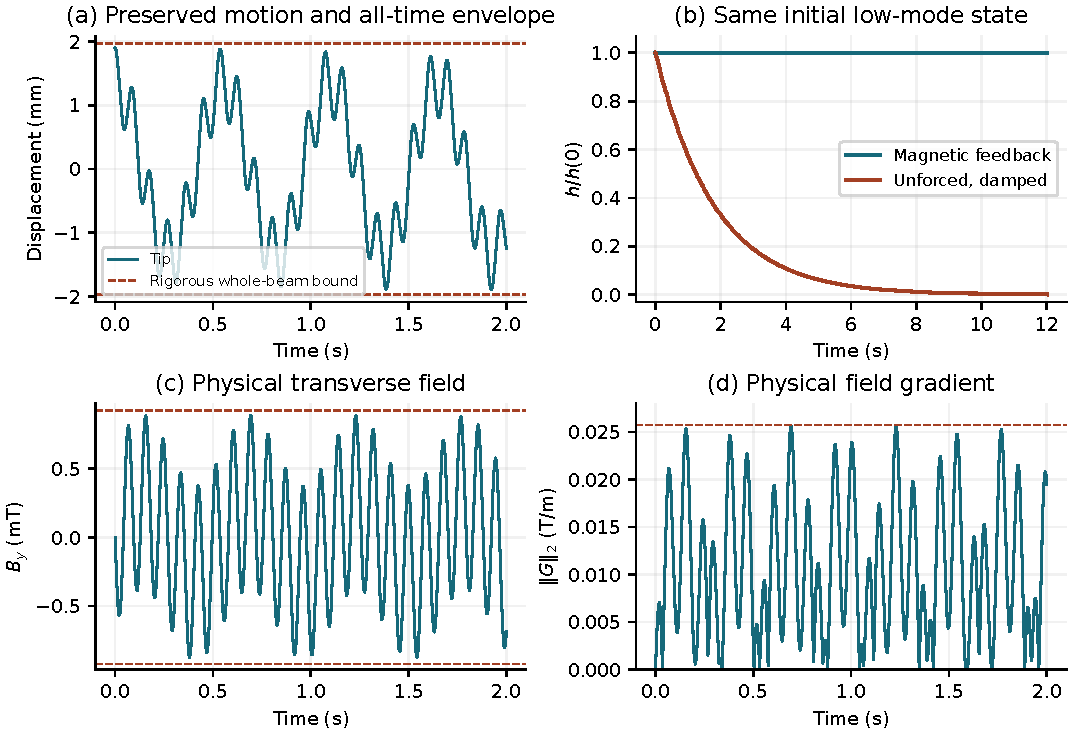
\includegraphics[width=\textwidth]{figures/fig_kam_magnetic_control.pdf}
\caption{Realizing the certified learned dynamics on all $64$ modes. The higher modes start at zero. Dashed envelopes include the startup transient and bound every phase and centreline point. Magnetic field and gradient jointly supply the force and torque; the passive comparison uses the same initial state without this feedback. Panels (a,c,d) show $2$ s and panel (b) shows $12$ s.}
\label{fig:core-kam-control}
\end{figure*}

\subsection{Frequency continuation and the clearance boundary}
To test where driven motion changes character, we vary a single sinusoidal transverse field from $1$ to $20$ mT and its frequency ratio $r=\omega_f/\omega_0$ from $0.7$ to $1.3$. The two-mode physical model is evaluated at $1{,}029$ independently initialized points and $686$ upward/downward continuation points. Each run discards $128$ forcing periods and diagnoses the next $64$ periods. All tested responses converge to forcing-periodic motion; their numerical Floquet spectral radii range from $0.803809$ to $0.889055$. These observations locate no quasiperiodic or chaotic transition within the sampled protocol. Large-deflection extrapolations are separately flagged, and this finite scan does not establish global absence of chaos or breakup of the conservative KAM tori.

A distinct practical boundary appears when periodic bending reaches the $4$ mm clearance. Solving for periodic responses with all $64$ modes gives threshold amplitudes of approximately $7.5005$, $1.91685$ and $8.7909$ mT at $r=0.9$, $1$ and $1.1$, respectively. These are numerical steady-response thresholds; the specified startup ramp can cross the clearance earlier. Supplement~\ref{S-sec:stability-boundary} reports the initial states, continuation protocol, transient thresholds, modal and temporal refinement, and independent full-model checks. The resonance boundary motivates a work constraint that covers transients as well as settled motion.

\subsection{Clearance beyond the invariant torus}
Tracking a prescribed path need not keep the state on a conservative torus. We therefore derive a clearance condition from the physical energy itself. For the clamped small-slope beam, $w(s)=\int_0^s(s-\xi)w_{ss}(\xi)\,d\xi$. Since the static magnetic energy is nonnegative, Cauchy--Schwarz gives
\begin{equation}
 |w(s,t)|^2\leq\frac{2s^3 E(t)}{3EI},\qquad
 E_c=\frac{3EIc^2}{2L^3},
\label{eq:core-clearance}
\end{equation}
where $c$ is the corridor half-width less the rod radius. Thus $E<E_c$ guarantees clearance of the entire centreline and its radius tube. This argument applies to sufficiently regular continuum solutions satisfying the power identity and separately to conforming Hermite finite-element solutions.

For a single transverse magnetic input, its actual power is $a_pB_y$, with $a_p=\mu\cos\vartheta\,\dot\vartheta$. Starting from a valid bound $\overline E_0\geq E(0)$, let $\dot W=a_pB_y$ and $W(0)=\overline E_0$. Nonnegative dissipation gives $E\leq W$. Choose $\overline E_0<E_{\max}<E_c$, and project the requested field onto
\begin{equation}
 |B_y|\leq B_{\max},\qquad
 a_pB_y\leq\kappa(E_{\max}-W),\quad\kappa>0.
\label{eq:core-governor}
\end{equation}
Zero field is feasible while $W\leq E_{\max}$. Moreover, \eqref{eq:core-governor} implies
$E_{\max}-W(t)\geq(E_{\max}-\overline E_0)e^{-\kappa t}$.
Together with \eqref{eq:core-clearance}, this proves all-time clearance under exact port measurement and command application. The result applies to driven trajectories through their supplied work, including motions away from a KAM torus; additional work ports or measurement errors must enter the same budget.

For a $4$ mm net clearance, $E_c=23.8565$ nJ. An energy budget $E_{\max}=0.95E_c$ bounds the centreline by $3.898718$ mm in continuous time. Under a $10$ mT sinusoidal request, the sampled peak falls from $5.14478$ mm without the governor to $3.14362$ mm with it; online COMSOL gives $3.143643$ mm. Supplement~\ref{S-sec:unifiedsafety} supplies the power derivation, an open-loop field-variation bound and refinement data.

\begin{figure*}[t]
\centering
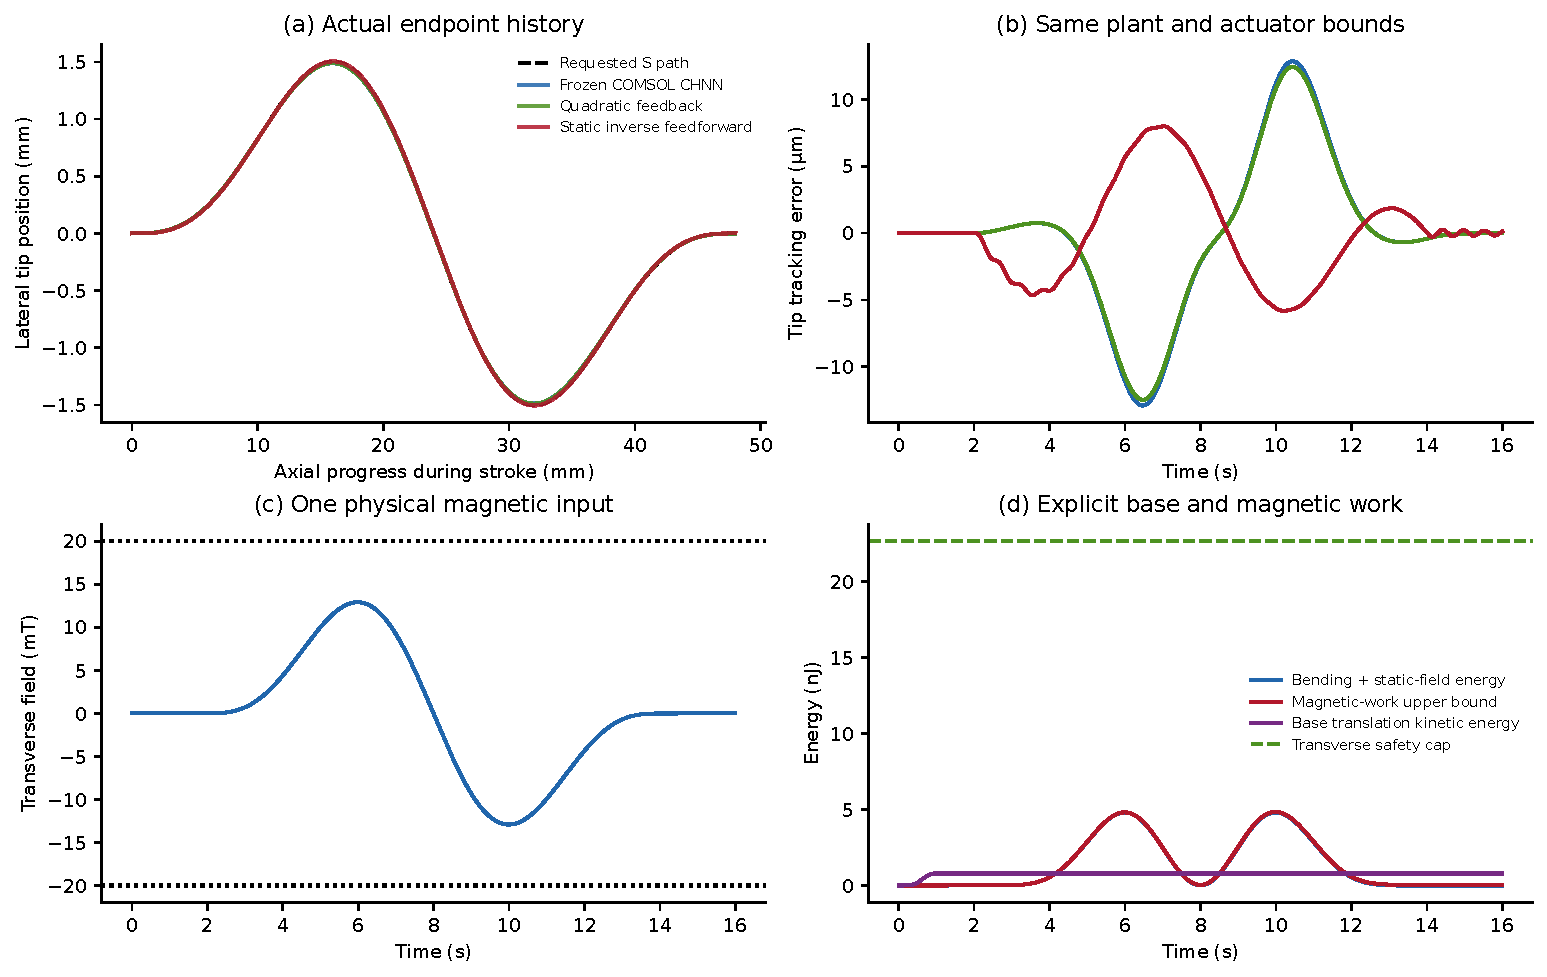
\includegraphics[width=\textwidth]{figures/fig_s_path_tracking.pdf}
\caption{S-shaped endpoint tracking through axial base feed and transverse magnetic actuation. The same full beam and input limits are used for the matched controls. Base work is included in the energy balance.}
\label{fig:core-s-path}
\end{figure*}

\subsection{Nonzero sensing, initialization and actuation tolerances}
The extremely narrow action tube in the KAM measure estimate is a proof domain, rather than an initialization tolerance. A separate physical-energy argument yields a nonzero operating tolerance about the exported finite Fourier reference. In the frozen full nodal model, let $Q(e)=\tfrac12 e_v^{\mathsf T}Me_v+\tfrac12 e_q^{\mathsf T}K_be_q$. The initialization set $Q(e)\leq5$ pJ implies a tip-position error below $56.006\,\mu$m; this is a projection of an energy ellipsoid, not a box of independently admissible coordinate errors.

For the two work ports, bound tip-angle, angular-rate and tip-velocity measurement errors by $1$ mrad, $0.01$ rad/s and $0.1$ mm/s. Allow $1\%$ multiplicative error in both applied inputs, together with additive errors of $0.5$ nN in force and $0.05\,\mu$T in field. A worst-case measured-power bound and a dissipation-based reserve of $0.096780$ nJ cover these additive errors over $4$ s. The resulting $22.66$ nJ energy cap bounds the whole centreline below $3.898405$ mm throughout that interval. Supplement~\ref{S-sec:operational-tolerances} gives the proof, directed-rounding certificate, actuator derating and full-model refinement. The governor can alter the requested motion substantially: this guarantee concerns clearance under the stated errors and does not preserve exact torus membership or certify tracking accuracy.

\subsection{Endpoint tracking and practical scope}
We next combine axial base translation with magnetic bending to trace an S-shaped endpoint path (Figure~\ref{fig:core-s-path}). The tip advances $48$ mm over a $12$ s stroke with lateral extrema $\pm1.5$ mm. Axial acceleration ends before bending begins, and the model has no axial drag or guide contact. With base kinetic energy and work accounted for separately, the transverse governor bounds clearance in the straight corridor (Supplement~\ref{S-sec:s-path}). The prescribed S shape is the moving endpoint trajectory.

The controller uses the two-mode Hamiltonian fitted to full-FE COMSOL trajectories, its full gradient and Hessian, observed low-mode projections and measured tip feedback, with coefficients fixed throughout the task. Table~\ref{tab:core-tracking} compares controllers on the same trajectory and plant with a $20$ mT field limit. The learned controller achieves $6.419\,\mu$m RMS error, while the known-physics inverse performs better on this slow nominal path. The modal-output comparison shows the benefit of using the measured tip in feedback.

\begin{table}[t]
\centering
\caption{Matched S-path controls. RMS errors use the $12$ s stroke; maxima use the complete $16$ s simulation.}
\label{tab:core-tracking}
\setlength{\tabcolsep}{3.5pt}
\begin{tabular}{lrr}
\toprule
Control & RMS ($\mu$m) & Max. ($\mu$m)\\
\midrule
CHNN, tip feedback & 6.419 & 12.907\\
Quadratic, tip feedback & 6.207 & 12.476\\
Static inverse feedforward & 4.124 & 8.005\\
CHNN, modal-output feedback & 25.308 & 41.544\\
\bottomrule
\end{tabular}
\end{table}

The learned command peaks at $12.9177$ mT and the centreline at $1.48892$ mm. The maximum recorded work-based energy estimate is $4.84997$ nJ, and the governor remains inactive for this request. An independent COMSOL replay of the field agrees with the predicted tip to within $4.038\times10^{-10}$ m. The replay tests this task's mechanical response; the torus experiment above additionally tests online feedback.

The resulting design guidance is to preserve fitted energy derivatives, check actuation rank and momentum invertibility, and budget all input work. The envelopes require the stated state estimates and local field/gradient authority. Device implementation requires calibrated hardware and verified error bounds; partial sensing, large rotations, flow and wall contact need corresponding extensions.

\clearpage
\section{Conclusion}
\label{sec:conclusion}
We connected an identified magnetic energy to numerical prediction, nonlinear persistence and physical actuation in four steps. The complex representation and classical central symplectic update preserve the model's structure; the approximation analysis carries nonzero identification error into the KAM hypotheses; and magnetic feedback realizes the resulting finite-amplitude torus in the damped full beam. The model-specific realization and lift yield explicit centreline, field and gradient bounds. Input-work control extends clearance guarantees to driven motions beyond that torus, with explicit nonzero initialization, sensing and actuation tolerances over a prescribed finite horizon. The frequency study identifies a resonance-induced clearance boundary; no chaotic transition is detected under its sampled protocol.

The numerical comparisons define the scope of this result: real and complex implementations have equivalent resolved accuracy, and the known-physics inverse performs best on the slow nominal tracking task. Extending the analysis to partial sensing, calibrated actuators and three-dimensional contact requires corresponding mechanical models and error bounds.

\section*{Data and code availability}
The supplied materials comprise two identified archives. Archive S1 is the complete computational record dated 2 October 2026, containing native COMSOL models, construction and learning code, trajectories, fitted coefficients and interval records. Archive S2, \texttt{S2\_citation\_revision\_20261008.zip}, contains the revised article and Supplement, the additional stability and tolerance studies, frozen inputs, raw numerical outputs and reproduction commands. The accompanying \texttt{reproducibility/ARTIFACT\_INDEX.md} identifies the archives and maps results to files and checksums; its source map separates full-FE identification from the two-mode integral data used for the KAM proof.
\section*{Declarations}
This work reports mathematical analysis and computer-generated mechanical data. No human, animal or in-orbit experiment was performed.
\begin{thebibliography}{99}
\bibitem[Abbott et~al.(2020)]{abbott}
Abbott JJ, Diller E and Petruska AJ (2020) Magnetic methods in robotics.
\textit{Annual Review of Control, Robotics, and Autonomous Systems} 3: 57--90.
\doi{10.1146/annurev-control-081219-082713}

\bibitem[Antman(2005)]{antman}
Antman SS (2005) \textit{Nonlinear Problems of Elasticity}. 2nd ed. Springer.
\doi{10.1007/0-387-27649-1}

\bibitem[Biasco and Chierchia(2018)]{biasco2018measure}
Biasco L and Chierchia L (2018) Explicit estimates on the measure of primary KAM tori.
\textit{Annali di Matematica Pura ed Applicata} 197(1): 261--281.
\doi{10.1007/s10231-017-0678-8}
\url{https://arxiv.org/abs/1612.01903}.

\bibitem[Bounemoura(2016)]{bounemoura2016torus}
Bounemoura A (2016) Non-degenerate Liouville tori are KAM stable.
\textit{Advances in Mathematics} 292: 42--51.
\doi{10.1016/j.aim.2016.01.012}
Preprint version used: \url{https://arxiv.org/abs/1412.0509v1}.

\bibitem[Bounemoura(2020)]{bounemoura}
Bounemoura A (2020) Positive measure of KAM tori for finitely differentiable Hamiltonians.
\textit{Journal de l'\'Ecole polytechnique -- Math\'ematiques} 7: 1113--1132.
\doi{10.5802/jep.137}

\bibitem[Chen et~al.(2022)]{chen2022}
Chen Y, Matsubara T and Yaguchi T (2022) KAM theory meets statistical learning theory:
Hamiltonian neural networks with non-zero training loss.
\textit{Proceedings of the AAAI Conference on Artificial Intelligence} 36(6): 6322--6332.
\doi{10.1609/aaai.v36i6.20582}

\bibitem[Chierchia and Koudjinan(2021)]{chierchia2021measure}
Chierchia L and Koudjinan CE (2021) V.~I.~Arnold's ``Global'' KAM theorem
and geometric measure estimates.
\textit{Regular and Chaotic Dynamics} 26(1): 61--88.
\doi{10.1134/S1560354721010044}
Preprint version used: \url{https://arxiv.org/abs/2010.13243v1}.

\bibitem[Das et~al.(2017)]{das2017quasiperiodicity}
Das S, Saiki Y, Sander E and Yorke JA (2017) Quantitative quasiperiodicity.
\textit{Nonlinearity} 30(11): 4111--4140.
\doi{10.1088/1361-6544/aa84c2}

\bibitem[Desai et~al.(2021)]{desai}
Desai SA, Mattheakis M, Sondak D, Protopapas P and Roberts SJ (2021)
Port-Hamiltonian neural networks for learning explicit time-dependent dynamical systems.
\textit{Physical Review E} 104: 034312. \doi{10.1103/PhysRevE.104.034312}

\bibitem[Duignan and Meiss(2023)]{duignan2023flows}
Duignan N and Meiss JD (2023) Distinguishing between regular and chaotic orbits
of flows by the weighted Birkhoff average.
\textit{Physica D: Nonlinear Phenomena} 449: 133749.
\doi{10.1016/j.physd.2023.133749}

\bibitem[Feng et~al.(1989)]{feng}
Feng K, Wu HM, Qin MZ and Wang DL (1989) Construction of canonical difference
schemes for Hamiltonian formalism via generating functions.
\textit{Journal of Computational Mathematics} 7(1): 71--96.
\url{https://computmath.cjoe.ac.cn/jcm/EN/Y1989/V7/I1/71}.

\bibitem[Francescon et~al.(2025)]{francescon2025shape}
Francescon V, Murasovs N, Lloyd P, Onaizah O, Chathuranga DS and Valdastri P (2025)
Closed-loop shape-forming control of a magnetic soft continuum robot.
\textit{IEEE Robotics and Automation Letters} 10(6): 6071--6078.
\doi{10.1109/LRA.2025.3565124}

\bibitem[Greydanus et~al.(2019)]{greydanus}
Greydanus S, Dzamba M and Yosinski J (2019) Hamiltonian neural networks.
In: \textit{Advances in Neural Information Processing Systems}, vol. 32.
\url{https://arxiv.org/abs/1906.01563}.

\bibitem[Hairer et~al.(2006)]{hairer}
Hairer E, Lubich C and Wanner G (2006) \textit{Geometric Numerical Integration:
Structure-Preserving Algorithms for Ordinary Differential Equations}. 2nd ed. Springer.
\doi{10.1007/3-540-30666-8}

\bibitem[Haro and Luque(2019)]{haro2019aposteriori}
Haro \`A and Luque A (2019) A-posteriori KAM theory with optimal estimates for
partially integrable systems. \textit{Journal of Differential Equations}
266(2--3): 1605--1674. \doi{10.1016/j.jde.2018.08.003}
Preprint version used: \url{https://arxiv.org/abs/1711.05515v1}.

\bibitem[Hornik(1991)]{hornik}
Hornik K (1991) Approximation capabilities of multilayer feedforward networks.
\textit{Neural Networks} 4(2): 251--257. \doi{10.1016/0893-6080(91)90009-T}

\bibitem[Kim et~al.(2019)]{kim}
Kim Y, Parada GA, Liu S and Zhao X (2019) Ferromagnetic soft continuum robots.
\textit{Science Robotics} 4(33): eaax7329. \doi{10.1126/scirobotics.aax7329}

\bibitem[NASA(2025)]{nasa}
NASA (2025) Risk of spaceflight associated neuro-ocular syndrome (SANS).
\href{https://www.nasa.gov/reference/risk-of-spaceflight-associated-neuro-ocular-syndrome-sans/}{NASA Human Research Program risk page}
(updated 16 May 2025; accessed 7 October 2026).

\bibitem[P\"oschel(2001)]{poschel}
P\"oschel J (2001) A lecture on the classical KAM theorem.
In: \textit{Proceedings of Symposia in Pure Mathematics}, vol. 69, pp. 707--732.
\doi{10.1090/pspum/069/1858551}
Preprint version used: \url{https://arxiv.org/abs/0908.2234v1} (Version 1.3, 2009).

\bibitem[Simo(1985)]{simo}
Simo JC (1985) A finite strain beam formulation. The three-dimensional dynamic problem.
Part I. \textit{Computer Methods in Applied Mechanics and Engineering} 49(1): 55--70.
\doi{10.1016/0045-7825(85)90050-7}

\bibitem[Tong et~al.(2025)]{tong2025navigation}
Tong D, Hao Z, Li J, Sun B, Liu M, Wang L and Huang W (2025)
Real-time simulation enabled navigation control of magnetic soft continuum robots in confined lumens.
\textit{Journal of the Mechanics and Physics of Solids} 203: 106198.
\doi{10.1016/j.jmps.2025.106198}

\bibitem[Trabelsi et~al.(2018)]{trabelsi}
Trabelsi C, Bilaniuk O, Zhang Y et~al. (2018) Deep complex networks.
In: \textit{International Conference on Learning Representations}.
\url{https://arxiv.org/abs/1705.09792}.

\bibitem[Zhang et~al.(2022)]{zhang}
Zhang SQ, Gao W and Zhou ZH (2022) Towards understanding theoretical advantages of
complex-reaction networks. \textit{Neural Networks} 151: 80--93.
\doi{10.1016/j.neunet.2022.03.024}
\href{https://www.lamda.nju.edu.cn/zhangsq/papers/2022-CRNet-NN.pdf}{Published version used for theorem numbering}.

\bibitem[Zhong et~al.(2020)]{zhong}
Zhong YD, Dey B and Chakraborty A (2020) Dissipative SymODEN: Encoding Hamiltonian
dynamics with dissipation and control into deep learning.
In: \textit{ICLR Workshop on Integration of Deep Neural Models and Differential Equations}.
\url{https://arxiv.org/abs/2002.08860}.
\end{thebibliography}

\end{document}
